\section{Introduction}
\label{sec:intro}

Latent diffusion models \citep{rombach2022high} have emerged as a leading framework and demonstrated great success in image synthesis \citep{flux2024,esser2024scaling}. They employ an autoencoder to project the images to the latent space to reduce the cost of diffusion models. For example, the predominantly adopted solution in current latent diffusion models \citep{rombach2022high,flux2024,esser2024scaling,chenpixart,chen2024pixart} is to use an autoencoder with a spatial compression ratio of 8 (denoted as f8), which converts 
images of spatial size $H\times W$ to latent features of spatial size $\frac{H}{8} \times \frac{W}{8}$. This spatial compression ratio is satisfactory for low-resolution image synthesis (e.g., $256 \times 256$). However, for high-resolution image synthesis (e.g., $1024 \times 1024$), further increasing the spatial compression ratio is critical, especially for diffusion transformer models \citep{peebles2023scalable, bao2023all} that have quadratic computational complexity to the number of tokens.

The current common practice for further reducing the spatial size is downsampling on the diffusion model side. For example, in diffusion transformer models \citep{peebles2023scalable, bao2023all}, this is achieved by using a patch embedding layer with patch size $p$ that compresses the latent features to $\frac{H}{8p} \times \frac{W}{8p}$ tokens. In contrast, little effort has been made on the autoencoder side. The main bottleneck hindering the employment of high spatial-compression autoencoders is the reconstruction accuracy drop. For example, Figure~\ref{fig:figure1_results} (a) shows the reconstruction results of SD-VAE \citep{rombach2022high} on ImageNet $256 \times 256$ with different spatial compression ratios. We can see that the rFID (reconstruction FID) degrades from 0.90 to 28.3 if switching from f8 to f64. 

This work presents \textbf{\modelfull (\modelshort)}, a new family of high spatial-compression autoencoders for efficient high-resolution image synthesis. By analyzing the underlying source of the accuracy degradation between high spatial-compression and low spatial-compression autoencoders, we find high spatial-compression autoencoders are more difficult to optimize (Section~\ref{sec:motivation}) and suffer from the generalization penalty across resolutions (Figure~\ref{fig:method_motivation} b). To this end, we introduce two key techniques to address these two challenges. First, we propose \textbf{Residual Autoencoding} (Figure~\ref{fig:method_arch}) to alleviate the optimization difficulty of high spatial-compression autoencoders. It introduces extra non-parametric shortcuts to the autoencoder to let the neural network modules learn residuals based on the space-to-channel operation. Second, we propose \textbf{Decoupled High-Resolution Adaptation} (Figure~\ref{fig:method_training_pipeline}) to tackle the other challenge. It introduces a high-resolution latent adaptation phase and a low-resolution local refinement phase to avoid the generalization penalty while maintaining a low training cost. 

With these techniques, we increase the spatial compression ratio of autoencoders to 32, 64, and 128 while maintaining good reconstruction accuracy (Table~\ref{tab:ae_main}). The diffusion models can fully focus on the denoising task with our \modelshort taking over the whole token compression task, which delivers better image generation results than prior approaches (Table~\ref{tab:diffusion_imagenet_main}). For example, replacing SD-VAE-f8 with our \modelshort-f64, we achieve \textbf{17.9$\times$} higher H100 training throughput and \textbf{19.1$\times$} higher H100 inference throughput on UViT-H \citep{bao2023all} while improving the ImageNet $512 \times 512$ FID from 3.55 to 3.01.  
We summarize our contributions as follows:

\vspace{-5pt}
\begin{itemize}[leftmargin=*]
\item We analyze the challenges of increasing the spatial compression ratio of autoencoders and provide insights into how to address these challenges.  
\item We propose Residual Autoencoding and Decoupled High-Resolution Adaptation that effectively improve the reconstruction accuracy of high spatial-compression autoencoders, making their reconstruction accuracy feasible for use in latent diffusion models. 
\item We build \modelshort, a new family of autoencoders based on our techniques. It delivers significant training and inference speedup for diffusion models compared with prior autoencoders. 
\end{itemize}

\begin{figure}[t]
    \centering
    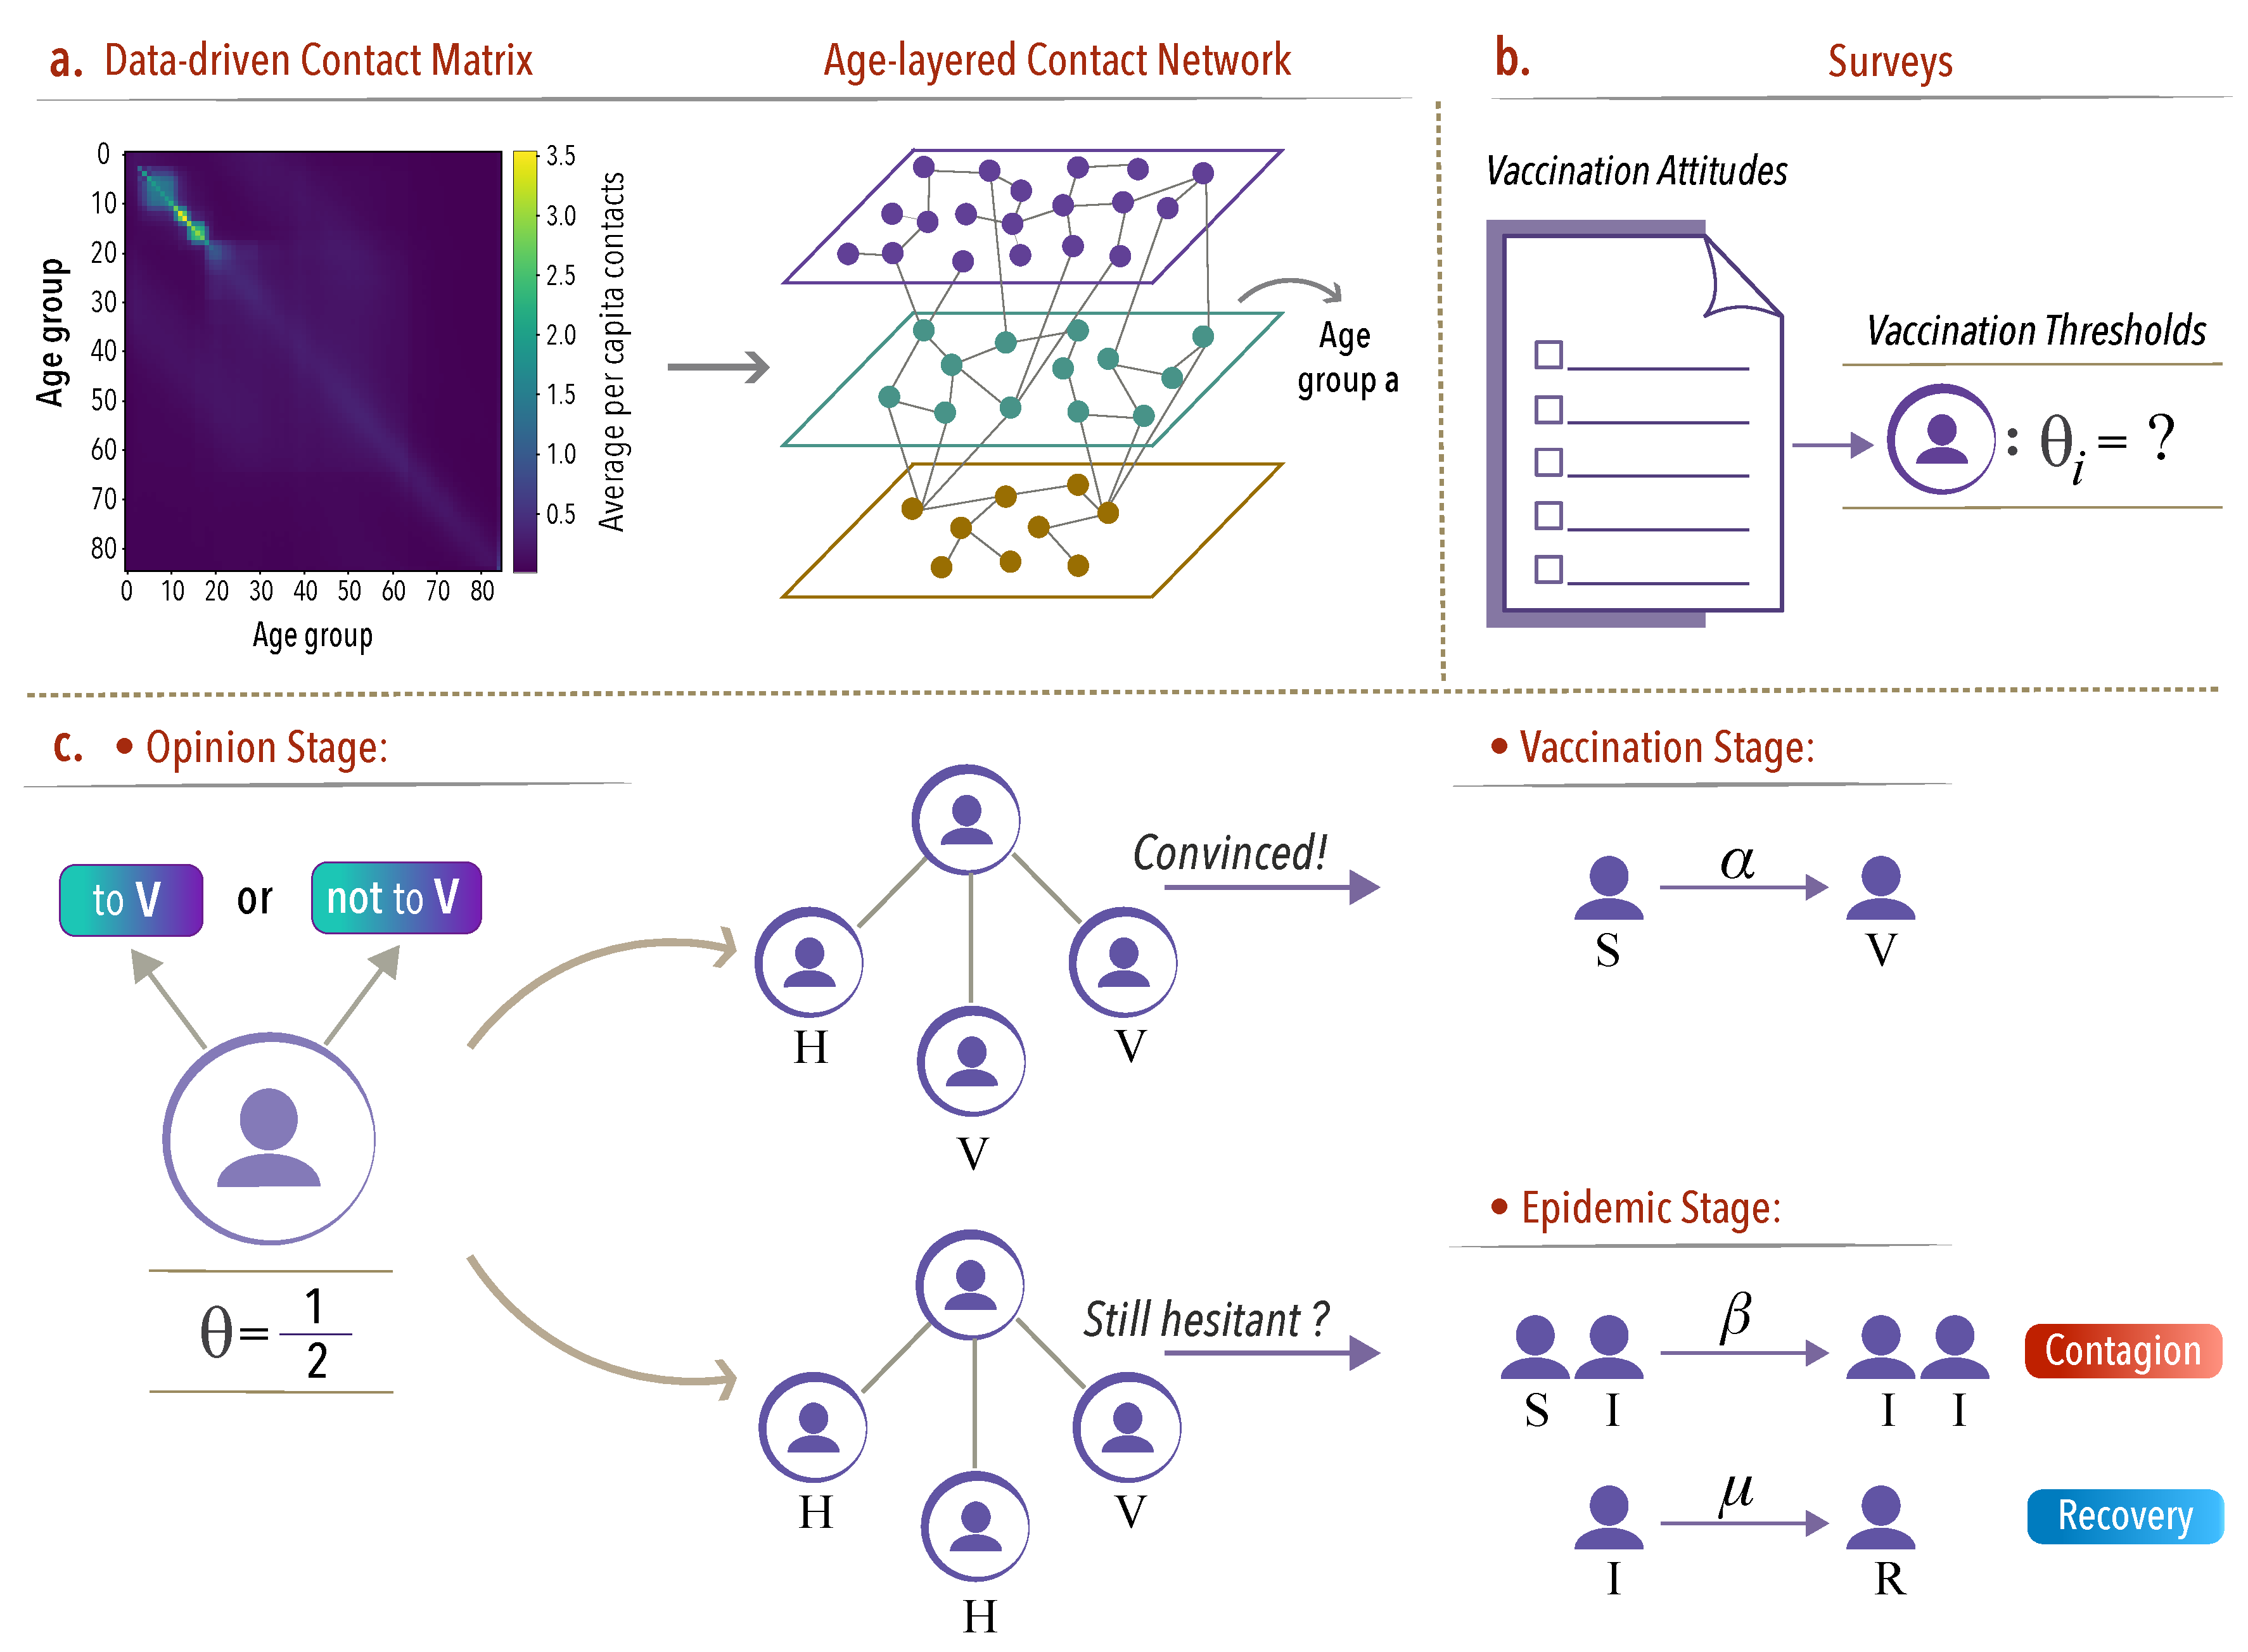
\includegraphics[width=1\linewidth]{figures/src/figure1.pdf}
    \vspace{-15pt}
    \caption{\modelshort accelerates diffusion models by increasing autoencoder's spatial compression ratio.}
    \vspace{-10pt}
    \label{fig:figure1}
\end{figure}


\begin{figure}[t]
    \centering
    \includegraphics[width=1\linewidth]{figures/src/figure1_results.pdf}
    \vspace{-15pt}
    \caption{\textbf{(a) Image Reconstruction Results on ImageNet 256$\times$256.} f denotes the spatial compression ratio. When the spatial compression ratio increases, SD-VAE has a significant reconstruction accuracy drop (higher rFID) while \modelshort does not have this issue. \textbf{(b) ImageNet 512$\times$512 Image Generation Results on UViT-S with Various Autoencoders.} p denotes the patch size. Shifting the token compression task to the autoencoder enables the diffusion model to focus more on the denoising task, leading to better FID. \textbf{(c) Comparison to SD-VAE-f8 on ImageNet 512$\times$512 with UViT Variants.} \modelshort-f64p1 provides 19.1$\times$ higher inference throughput and 0.54 better ImageNet FID than SD-VAE-f8p2 on UViT-H.}
    \vspace{-10pt}
    \label{fig:figure1_results}
\end{figure}

